\chapter{Introduction}

Anyone who ever moved places knows the amazing difference between the sound of talking inside an empty room
as opposed to talking in that same room once it's filled with furniture.
Acoustics as a field has long been dedicated to exploring these kinds of differences,
as well as developing methods to ensure that a room's acoustics fit its purpose.
\newline
As with all fields, software tools have been developed to aid in adjusting a room's acoustics.
Several methods have been developed that allow an engineer to simulate the sound of a planned room before building and furnishing it,
letting them check whether the acoustics hold up to their intended requirements.
\newline
The two most common methods of simulation are numeric and geometric approaches.
Numeric approaches work by getting the equation representing the wave's propagation in the room,
then calculating a solution to it numerically.
This leads to the most accurate results, but has a high computation cost attached to it,
making it less viable for real-world uses.
\newline
Geometric methods instead model a sound wave as a large set of individual rays originating from the same spot,
then simulate them bouncing through the room,
similarly to how light is modelled in graphics ray tracers.
This works fine for sounds at small wave lengths/high frequencies,
but introduces errors for lower frequencies as a sound's wave properties are entirely discarded.
In turn, geometric methods are much faster than numeric approaches,
to a point where a room's acoustics can be simulated in real time~\cite{Cha08}.
At time of writing, most commercially available acoustics simulation tools use ray tracing or similar geometric methods~\cite{Th17}.
\newline
Both of these methods can of course also be used to simulate entirely hypothetical rooms without any intent to build them,
or rooms that can't exist in the real world to begin with,
which can help physicists study properties of these theoretical places that can then be applied to real ones.
\newline
An example for a case that would be interesting to study but near impossible to measure in real life
would be the acoustics of a rapidly rotating room.
In order to differ from the echo the room creates while static,
the room's rotation would need to reach a velocity at least one order of magnitude below the speed of sound.
Building such a rotating room in the real world may be possible at a small scale,
but becomes exponentially harder the bigger the room gets.
\newline
In order to simulate such a room, the simulation would need to be able to account for
the walls of the room moving while the sound wave itself is traversing the scene.
This is mostly unexplored thus far.
Bilibashi et al.~\cite{BVD20} have explored simulating rays bouncing between a set of moving points, namely cars,
but their approach is not viable for a full room acoustics simulation.
\newline
Existing simulations have only concerned themselves with static scenes.
% TODO cite EAR
For dynamic scenes, existing tools such as EAR and research such as that by Chandak et al.~\cite{Cha08}
work around having to account for movement by taking a static version of the scene at a given time
and bouncing rays through that instead,
then repeating this process for every point in time at which acoustics are simulated.
\newline
This works well in most cases, but leads to problems when objects in the room move fast enough
that the distance they would travel in the time a ray is bouncing through the scene becomes significant.
To alleviate this problem, this thesis proposes a method to simulate the acoustics of a moving room without errors.

\iffalse
Both EAR and Chandak et al.\ approach the simulation of moving scenes by taking a static version of the scene
at the time rays are emitted to create an impulse response,
then bouncing rays through this static snapshot.
This approach will be called the snapshot method in this thesis.
\newline
The snapshot method comes with a few advantages:
As the snapshot is just a static scene,
the same well-explored and -optimised bouncing logic used for static scenes can be copied without changes.
Also, crucially, knowledge of how the scene will move over the time the ray spends bouncing around it is not required.
All data necessary to simulate the bouncing is available at the time the ray is emitted,
without a need for information on how the scene will continue to move.
This is especially helpful for real-time simulation of dynamic scenes, as data about how the scene will continue to move is not
fully known at runtime.
\newline
\begin{figure}\label{SnapshotExplain}
    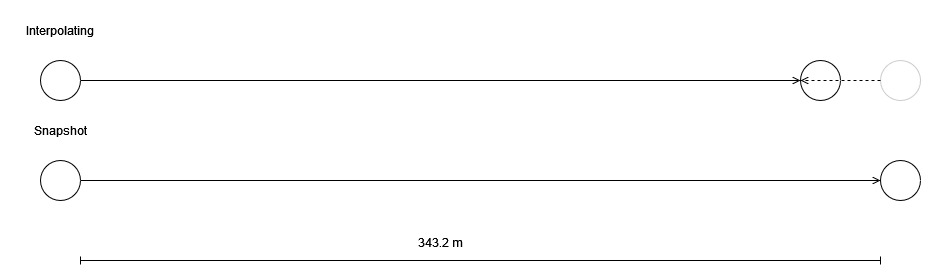
\includegraphics[width=\linewidth]{images/snapshot_explain.jpg}
    \caption{Difference between ray travelling distance using the newly developed interpolating method (top) as opposed to the snapshot method (bottom). In the interpolated version, the ray only travels part of the distance as the receiver travels the remainder.}
\end{figure}
The major downside of this snapshot approach is that it tends to introduce errors when objects or receivers move at high speeds.
As a simple example case, take the scene described in~\ref{SnapshotExplain}:
A receiver starts 343 meters away from an emitter and moves towards it at 1/9th the speed of sound, roughly 38 meters per second
(137.2 kilometers per hour, a speed most modern cars can reach without problems).
\newline
Using the snapshot approach, a ray traveling directly from emitter to receiver would arrive after travelling the full 343 meters,
taking 1 second for it to arrive at the receiver.
In actuality, in the time the ray takes to travel the first 90\% of that distance,
the receiver has already travelled the remaining 10\%, making for a response time of 0.9 seconds rather than 1 second.
\fi

\section{Scope of This Thesis}

This thesis proposes a method to simulate rays bouncing through arbitrary scenes with moving receivers and/or objects,
assuming all movement within the scene is known at time of calculation.
An improved way of checking for intersections between rays and objects is developed, accommodating for this new requirement.
Optimisations are evaluated and a time-based chunking method is developed to avoid needless intersection checks.
Additionally, a method is developed to to losslessly and efficiently store the multiple impulse responses created by re-calculating
the impulse responses for different points in time.
The goal of this research is to lay the groundwork to allow accurate simulation of acoustics in moving rooms.
Three test cases are developed for this and compared to an implementation more akin to existing methods:
An empty scene with the sound receiver approaching the sound emitter at 1/9th the speed of sound,
a square room rapidly rotating
and a large, L-shaped room also rapidly rotating around one of its ends, with the receiver and emitter both sitting in said end.
\newline
Not within the scope of this thesis is development of a fully accurate simulator
including effects such as the differing bouncing behaviour sound waves show at different frequencies.
Only a proof of concept that shows that the idea of this new simulation method works is developed.
\newline
Side effects of moving scenes, such as sounds emitted by moving objects, are also discarded as they are irrelevant to
the changed intersection logic.
A note-worthy side effect that gets ignored is mass inertia:
The example case where this would become relevant is the inside of a linearly moving enclosed room, such as a driving car.
Due to mass inertia, sound waves travelling inside this moving rome behave the same as if the car stood still.
Since this effect is only relevant in a niche scenario and it can be simulated using a method that ignores movement entirely,
it can be ignored for this research.
\newline
Real-time applications cannot use this proposed method as it requires knowledge of objects' future movements ahead of time.
Further research is required to develop an alternative method for real-time or dynamic simulations.
A real-time approach could work by not calculating the rays' entire movements at emission time,
but instead keeping track of all moving rays and incrementally continuing their journey through the now updated scene
at recurring intervals.

\section{Outline}

Fundamentals ch2
\newline
intersecion checks ch3
\newline
chunking ch4
\newline
irs ch5
\newline
eval ch6